\documentclass[preview]{standalone}
\usepackage{pgfplots}
\pgfplotsset{compat=1.16}
\begin{document}

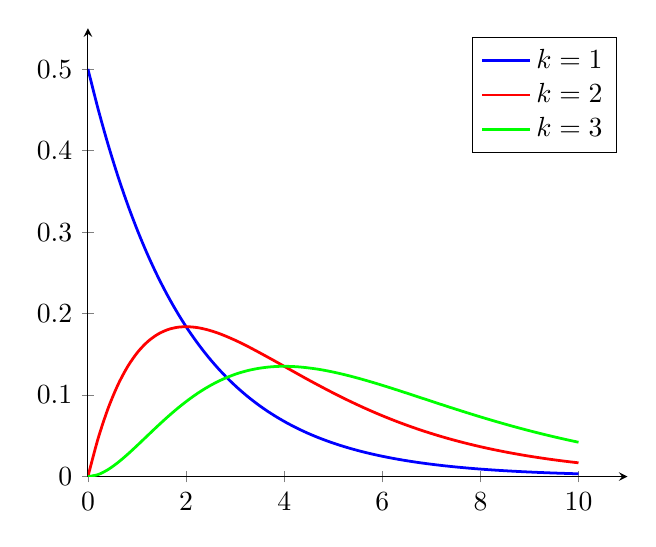
\begin{tikzpicture}[
    declare function={gamma(\z)=
    (2.506628274631*sqrt(1/\z) + 0.20888568*(1/\z)^(1.5) + 0.00870357*(1/\z)^(2.5) - (174.2106599*(1/\z)^(3.5))/25920 - (715.6423511*(1/\z)^(4.5))/1244160)*exp((-ln(1/\z)-1)*\z);},
    declare function={gammapdf(\x,\k,\theta) = \x^(\k-1)*exp(-\x/\theta) / (\theta^\k*gamma(\k));}
]

\begin{axis}[
    axis lines=left,
    enlargelimits=upper,
    xtick={0, 2,...,10},
    samples=50,
    legend entries={$k=1$,$k=2$,$k=3$}
]
\addplot [smooth, domain=0:10, blue, line width=1] {gammapdf(x,1,2)};
\addplot [smooth, domain=0:10, red, line width=1 ] {gammapdf(x,2,2)};
\addplot [smooth, domain=0:10, green, line width=1] {gammapdf(x,3,2)};
\end{axis}
\end{tikzpicture}
\end{document}